\section{System Architecture}
\label{sec:SystemArchitecture}
This section explores the system architecture of the application, which adopts a microfrontend architecture to separate different business domains into distinct, independently developed, and deployed microfrontends. We present the various microfrontends and other components that make up the system, explaining the rationale behind these segmentation decisions. Figure \ref{fig:app-architecture} illustrates this architecture using a UML component diagram.
\begin{figure}[h]  
    \centerline{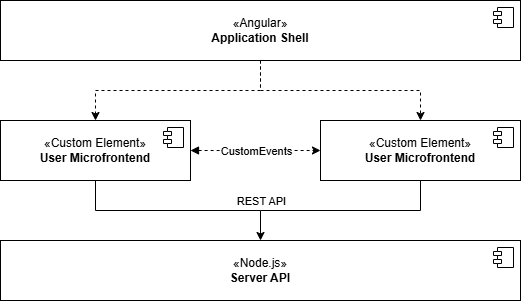
\includegraphics[width=.75\textwidth]{images/app-architecture.png}}  
    \caption[Application architecture component diagram]{Component diagram of the application architecture}  
    \label{fig:app-architecture}  
\end{figure}

\subsection{Application Shell}
The Application Shell is the core of the application; it functions as an orchestrator for all microfrontends. Based on the current route, it loads and renders the appropriate microfrontends. It handles all global functionality—such as routing, theme settings, and language switching—in a centralized manner. It passes any necessary data down to the microfrontends, such as the current language (English or Slovak) or customization options. Common elements, such as navigation and settings, are also located here. Additionally, it renders the dashboard page by combining multiple microfrontends into a single unified view.

The reasoning behind this is clear: we wanted to keep all common elements in one place and handle global functionality centrally. This greatly reduces code redundancy and improves maintainability. The Application Shell only needs to know the URLs where the microfrontends are hosted, as well as their HTML element names and attributes, and it can be developed and deployed independently.

\subsection{User Microfrontend}
This microfrontend is primarily responsible for user management functionality within the application. It handles user management through CRUD operations (Create, Read, Update, Delete) and displays users in a table format. It is a standalone page within the application, rendered independently by the Application Shell. It receives several attributes from the Application Shell: the first is \texttt{language}, which the microfrontend should use (default: English); the second is \texttt{theme}, either light or dark; and the third is a boolean attribute, \texttt{compact}, which defaults to \texttt{false}. If this attribute is set to \texttt{true}, the microfrontend switches to a compact mode, displaying only a simple list of new users and a monthly user count graph for dashboard purposes, allowing it to be displayed alongside other microfrontends.

Clicking on a user in the list selects them; clicking again deselects them. This action triggers an event to notify other microfrontends about the selection. Additionally, the microfrontend listens for events related to task selection or deselection—in such cases, it displays only users assigned to the selected task.

By following this approach, the user management microfrontend remains completely isolated from the rest of the system. It is reusable, customizable, and serves a single business domain. The only information it needs to function correctly is the names of the events it should listen to.

\subsection{Task Microfrontend}
This microfrontend is primarily responsible for task management. Similar to the user management microfrontend, it supports task CRUD operations (Create, Read, Update, Delete) and displays tasks using a Kanban board. It functions as a standalone page within the application and is rendered independently by the Application Shell. It receives the same attributes from the Application Shell as the user microfrontend: \texttt{language}, \texttt{theme}, and \texttt{compact}.

When the \texttt{compact} mode is enabled, the microfrontend displays only a simplified view, including a list of new tasks and a monthly task count graph, making it suitable for use within the dashboard. Clicking on a task selects or deselects it, triggering an event to notify other microfrontends of the selection. Additionally, this microfrontend listens for user selection and deselection events. When a user is selected, it filters the displayed tasks to show only those assigned to the selected user.

The rationale for this design follows the same principles as those applied to the user management microfrontend: modularity, reusability, and isolation of concerns.

\subsection{Backend}
In a real-world microfrontend-based application, each microfrontend would ideally use its own microservice and a database. However, given the scope and constraints of this thesis and extensive existing research on microservices and backend architectures, our focus will remain on the frontend implementation. As a result, we will use a simple, lightweight monolithic backend to support the application's functionality.
